\documentclass[12pt,a4paper]{article}
\usepackage[margin=1in]{geometry}
\usepackage{graphicx}
% Figures live in report/figures/; Architecture.png is shared with the README in img/
\graphicspath{{figures/}{../img/}}
\usepackage{booktabs}
\usepackage{amsmath}
\usepackage{hyperref}
\usepackage{xcolor}
\usepackage{float}
\usepackage{caption}
\usepackage{subcaption}
\usepackage{listings}
\usepackage{enumitem}
\usepackage{titlesec}
\usepackage{fancyhdr}
\usepackage{multirow}
\usepackage{array}
\usepackage{microtype}
\usepackage{parskip}
\usepackage{mdframed}

\hypersetup{colorlinks=true,linkcolor=blue!70!black,citecolor=green!50!black,urlcolor=blue}
\definecolor{codeblue}{RGB}{37,99,235}
\definecolor{highlight}{RGB}{254,243,199}
\definecolor{bestrow}{RGB}{209,250,229}

\lstset{
  basicstyle=\ttfamily\small,
  breaklines=true,
  frame=single,
  backgroundcolor=\color{gray!8},
  keywordstyle=\color{codeblue}\bfseries,
  commentstyle=\color{gray},
  rulecolor=\color{gray!30}
}

\pagestyle{fancy}
\fancyhf{}
\rhead{\small VidyaRAG — Multimodal NPTEL Lecture Retrieval}
\lhead{\small Sourav Nath, IIIT Hyderabad}
\cfoot{\thepage}
\renewcommand{\headrulewidth}{0.4pt}

\titleformat{\section}{\large\bfseries\color{codeblue}}{{\thesection}}{1em}{}[\titlerule]
\titleformat{\subsection}{\normalsize\bfseries}{{\thesubsection}}{1em}{}

\newcolumntype{C}[1]{>{\centering\arraybackslash}p{#1}}

\begin{document}

% ─────────────────────────────────────────────
%  TITLE PAGE
% ─────────────────────────────────────────────
\begin{titlepage}
\centering
\vspace*{1.5cm}
{\Huge\bfseries VidyaRAG\par}
\vspace{0.4cm}
{\Large Multimodal Hybrid Retrieval over NPTEL Lecture Videos\par}
\vspace{0.3cm}
{\large\color{gray} BGE-large $\cdot$ FAISS $\cdot$ BM25 $\cdot$ RRF $\cdot$ Cross-Encoder Reranking\par}
\vspace{1.5cm}
\hrule height 1pt
\vspace{0.8cm}
{\large\bfseries Sourav Nath\par}
\vspace{0.2cm}
{\normalsize International Institute of Information Technology -- Hyderabad\par}
{\normalsize \texttt{sourav.nath@students.iiit.ac.in}\par}
\vspace{0.6cm}
\hrule height 0.4pt
\vspace{0.8cm}
{\normalsize June 2026\par}
\vspace{1cm}

\begin{mdframed}[backgroundcolor=highlight,linecolor=orange!60,linewidth=1pt]
\centering
\textbf{Key Result:} MRR = \textbf{0.8259} $\;\cdot\;$ Recall@10 = \textbf{0.9643}\\
Evaluated on 84 human-annotated queries across 9 NPTEL CS courses
\end{mdframed}

\vspace{1cm}
\begin{tabular}{ll}
\textbf{Demo:} & \url{https://huggingface.co/spaces/SouravNath/vidyarag} \\
\textbf{Code:} & \url{https://github.com/Sourav-Nath-01/vidyarag} \\
\end{tabular}
\end{titlepage}

% ─────────────────────────────────────────────
%  TABLE OF CONTENTS
% ─────────────────────────────────────────────
\tableofcontents
\newpage

% ─────────────────────────────────────────────
%  ABSTRACT
% ─────────────────────────────────────────────
\begin{abstract}
We present \textbf{VidyaRAG}, a multimodal semantic search system over NPTEL lecture transcripts and slide content. The system combines dense retrieval using BGE-large-en-v1.5 embeddings with BM25 sparse retrieval, fused via Reciprocal Rank Fusion (RRF), and reranked using a cross-encoder. A novel slide-boundary chunking strategy (C3) is introduced that detects lecture slide transitions using OCR Jaccard similarity between consecutive segments. Evaluated on 84 human-annotated queries across 9 CS disciplines, the full system achieves MRR\,=\,0.8259 and Recall@10\,=\,0.9643, representing an \textbf{84.4\%} improvement over the fixed-window baseline in MRR. A rigorous 9-experiment ablation study isolates the contributions of OCR fusion, BM25 hybrid retrieval, and chunking strategy. The system is deployed as a live Streamlit application on Hugging Face Spaces with YouTube deep-link results.
\end{abstract}

\vspace{0.3cm}
\noindent\textbf{Keywords:} Information Retrieval, Retrieval-Augmented Generation, Multimodal RAG, Hybrid Search, BM25, FAISS, Cross-Encoder, Lecture Retrieval, NPTEL, OCR, Whisper ASR.

\newpage

% ─────────────────────────────────────────────
%  1. INTRODUCTION
% ─────────────────────────────────────────────
\section{Introduction}

NPTEL (National Programme on Technology Enhanced Learning) is one of the largest repositories of educational video content in India, hosting thousands of hours of lecture recordings across science and engineering disciplines. However, learners have no way to semantically search within these lectures -- they can only browse by course or manually scrub through video timestamps.

This project addresses that gap by building a \textbf{production-ready, multimodal semantic search system} that indexes both Whisper ASR transcripts and Tesseract OCR slide content, enabling natural language queries like \emph{"explain backpropagation"} or \emph{"BST insertion algorithm"} to return precise lecture segments with YouTube deep-links.

\subsection{Problem Statement}

Given a natural language query $q$, retrieve the top-$K$ lecture segments $\{s_1, \ldots, s_K\}$ from a corpus $\mathcal{C}$ of 9 NPTEL courses, ranked by relevance, such that the correct segment (verified by a human annotator against a timestamp) appears within the top-$K$ results.

\subsection{Contributions}

\begin{itemize}[leftmargin=1.5em]
  \item \textbf{Novel C3 chunking}: A slide-boundary detection algorithm using OCR Jaccard similarity to place chunk boundaries precisely at slide transitions.
  \item \textbf{Multimodal indexing}: ASR transcript + OCR slide text fused into a single passage for both dense and sparse retrieval.
  \item \textbf{Hybrid retrieval pipeline}: FAISS (BGE-large) + BM25 fused via RRF, followed by cross-encoder reranking.
  \item \textbf{Rigorous ablation}: 9 system experiments + 6 chunk-parameter sensitivity variants evaluated on 84 human-annotated queries.
  \item \textbf{Deployed system}: Live public demo on HF Spaces, FastAPI REST endpoint, and full unit test suite.
\end{itemize}

\newpage
% ─────────────────────────────────────────────
%  2. RELATED WORK
% ─────────────────────────────────────────────
\section{Related Work}

\subsection{Dense Retrieval}
Dense retrieval models such as DPR \cite{karpukhin2020dpr} encode queries and passages into shared embedding spaces using bi-encoders. BAAI/BGE-large-en-v1.5 \cite{bge2023} represents the current state-of-the-art for English dense retrieval, achieving top performance on BEIR benchmarks through contrastive pre-training on large corpora.

\subsection{Sparse Retrieval}
BM25 \cite{robertson2009probabilistic} remains a competitive sparse retrieval baseline, particularly for domain-specific lexical matching. Hybrid systems combining dense and sparse retrieval consistently outperform either alone \cite{luan2021sparse}.

\subsection{Reciprocal Rank Fusion}
RRF \cite{cormack2009reciprocal} is a rank fusion technique that combines result lists from multiple retrieval systems without score calibration. Given ranked lists $R_1, \ldots, R_m$ and a constant $k=60$:
\[
  \text{RRF}(d) = \sum_{i=1}^{m} \frac{1}{k + \text{rank}_i(d)}
\]

\subsection{Cross-Encoder Reranking}
Two-stage retrieval (retrieve-then-rerank) using cross-encoders \cite{nogueira2019passage} significantly improves precision. The cross-encoder jointly encodes query and passage, enabling fine-grained relevance scoring at the cost of latency, making it suitable only for a small candidate set.

\subsection{Multimodal Lecture Retrieval}
Prior work on lecture retrieval \cite{pan2017lecture} has focused on ASR-only retrieval. Fusing slide OCR content with ASR transcripts for hybrid search in educational video is, to our knowledge, underexplored in the NPTEL domain.

\newpage

% ─────────────────────────────────────────────
%  3. SYSTEM ARCHITECTURE
% ─────────────────────────────────────────────
\section{System Architecture}

\begin{figure}[H]
  \centering
  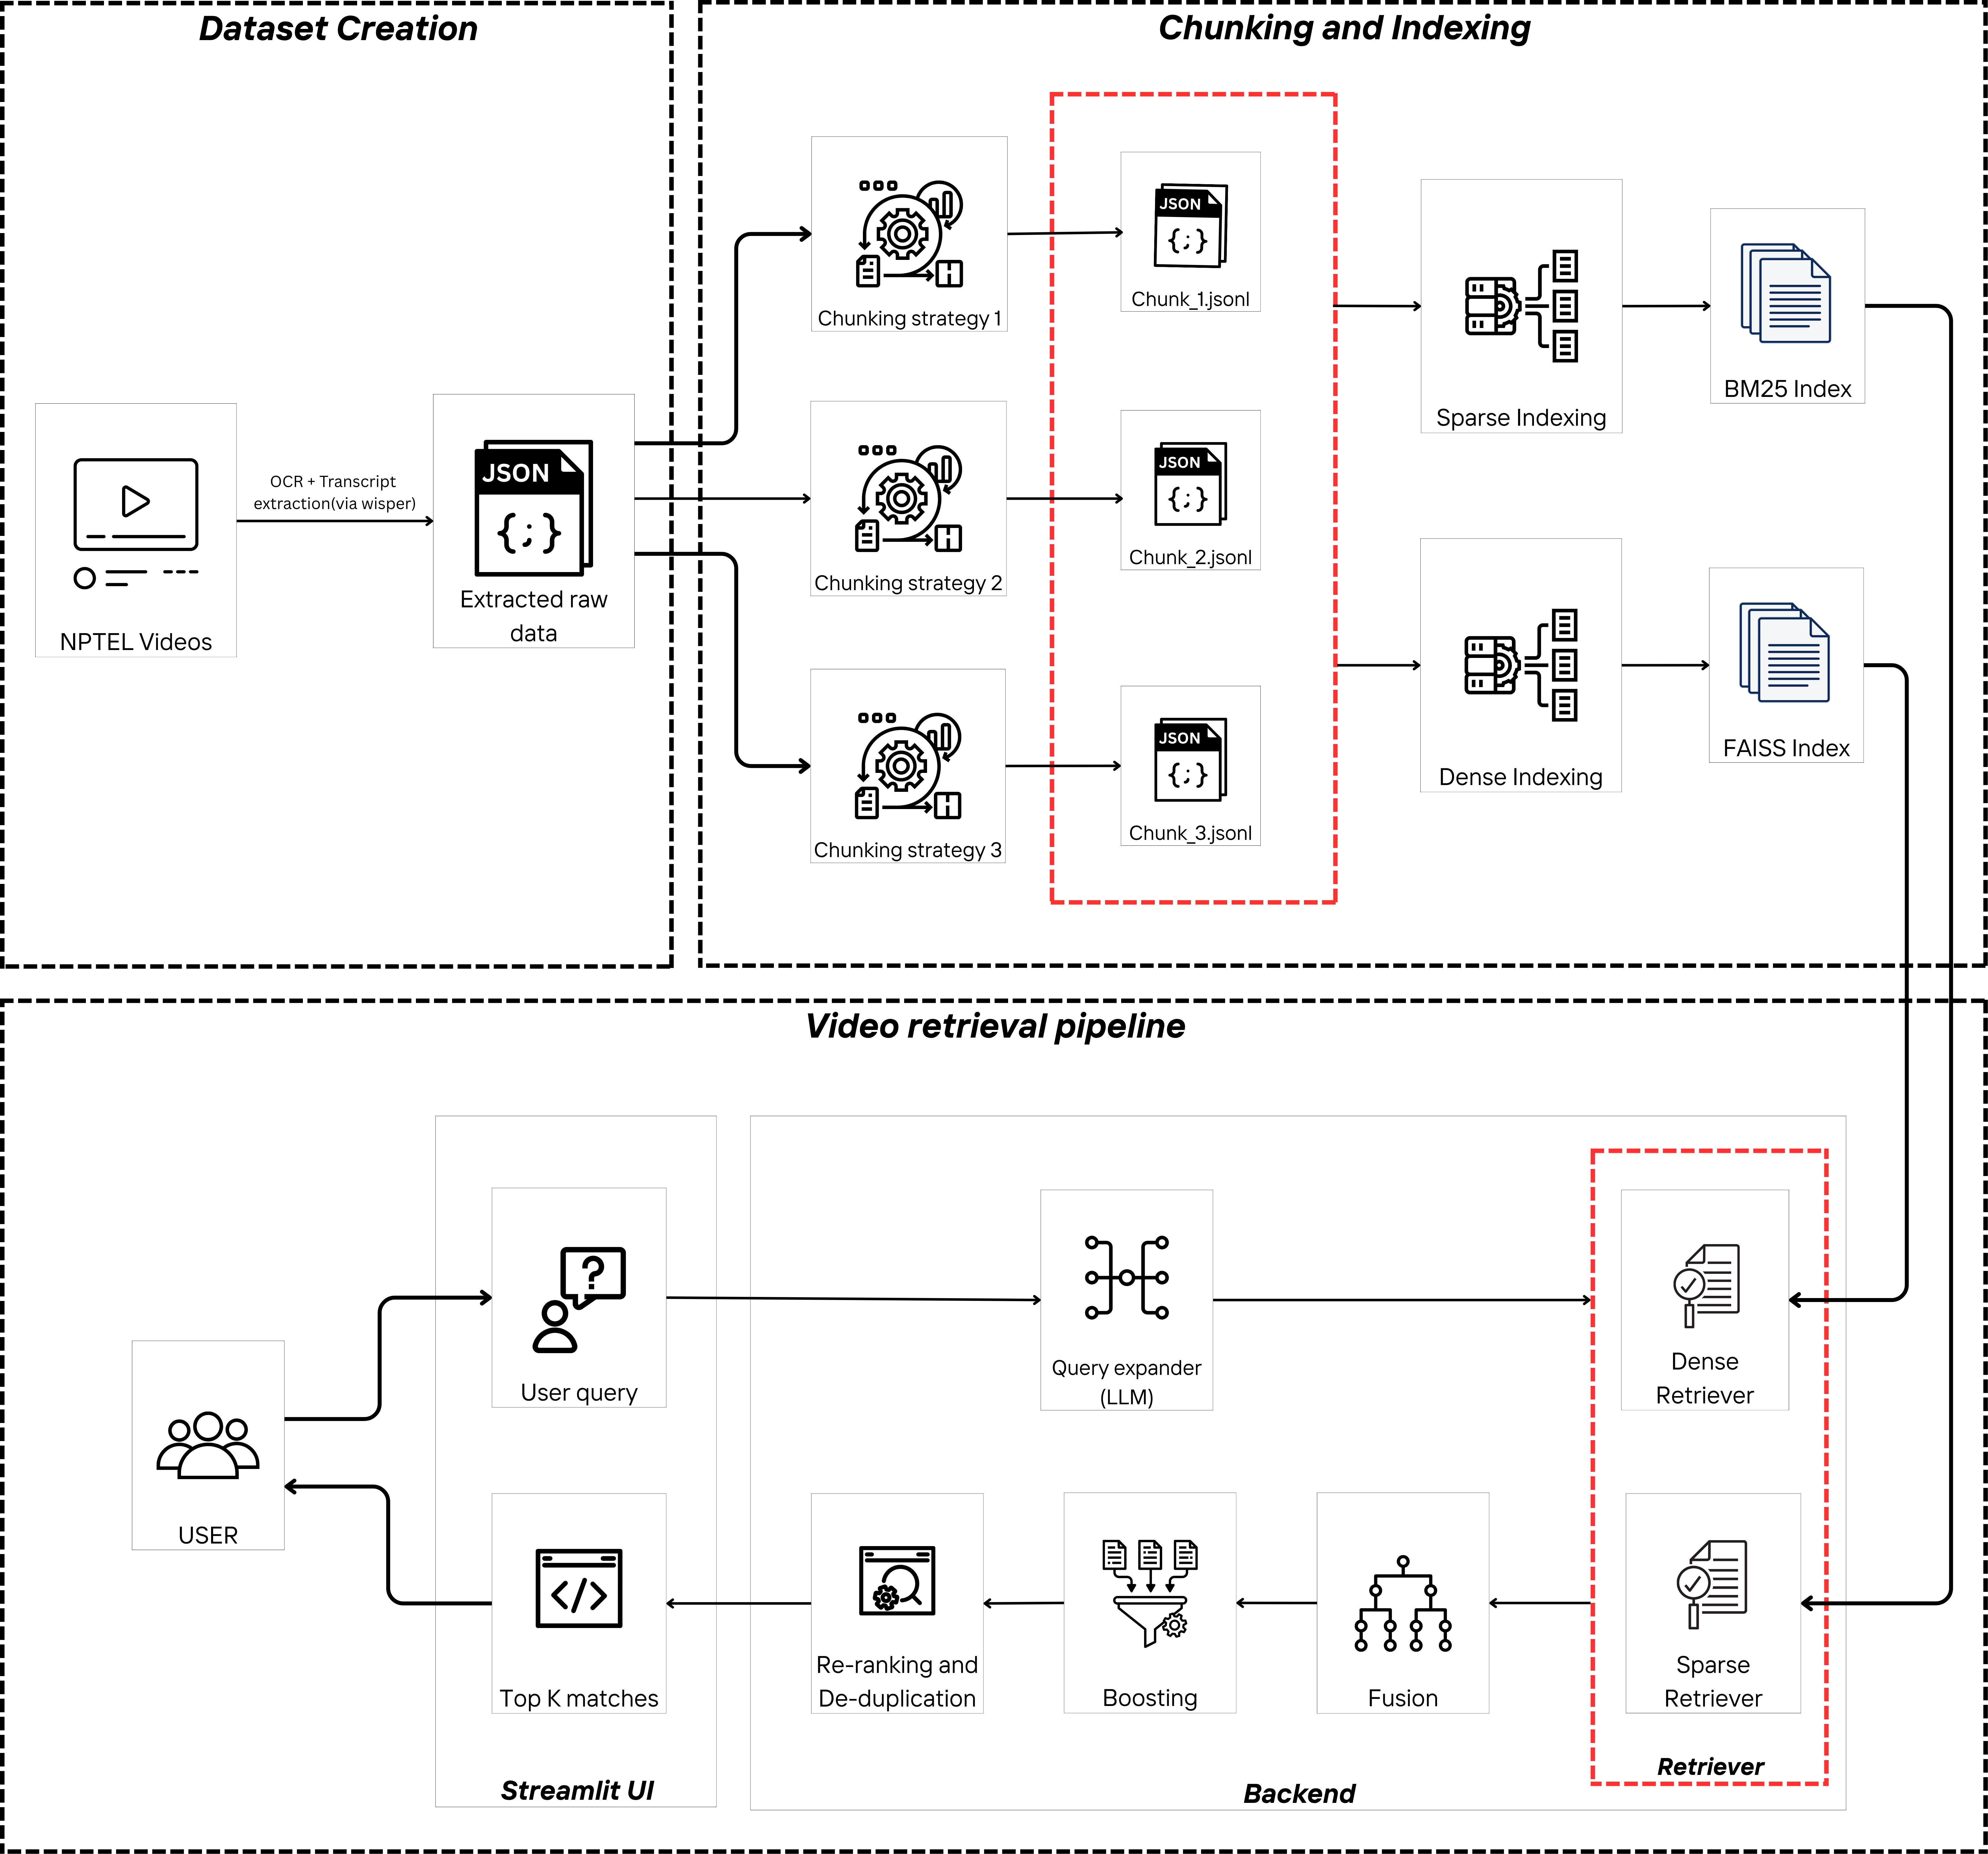
\includegraphics[width=0.92\textwidth]{Architecture.png}
  \caption{VidyaRAG system architecture showing the data pipeline (left) and retrieval pipeline (right).}
  \label{fig:arch}
\end{figure}

The system consists of two major pipelines: an offline \textbf{indexing pipeline} and an online \textbf{retrieval pipeline}.

\subsection{Offline Indexing Pipeline}

\begin{enumerate}[leftmargin=1.5em]
  \item \textbf{ASR Transcription}: Whisper (OpenAI) generates word-level transcripts with timestamps for each lecture video.
  \item \textbf{OCR Extraction}: Tesseract extracts text from lecture slide frames at 1 FPS. Frames are associated with the closest transcript segment by timestamp.
  \item \textbf{Chunking} (C1/C2/C3 — see Section~\ref{sec:chunking}): Transcripts are segmented into retrievable units.
  \item \textbf{Passage Construction}: Each segment is rendered as a structured passage:
    \begin{lstlisting}
Passage: [course] [lecture_title] | [transcript] | Slide: [ocr_text]
    \end{lstlisting}
  \item \textbf{Dense Embedding}: BGE-large-en-v1.5 encodes each passage into a 1024-dimensional vector. Stored in a FAISS \texttt{IndexFlatIP} index.
  \item \textbf{BM25 Indexing}: Tokenized passages (stopword-filtered, stemmed) indexed via \texttt{rank-bm25}.
\end{enumerate}

\subsection{Online Retrieval Pipeline}

\begin{enumerate}[leftmargin=1.5em]
  \item \textbf{Optional LLM Query Analysis} (Ollama, Llama 3.2:3b): Intent classification (code / theoretical / conceptual) and query expansion.
  \item \textbf{Query Embedding}: BGE-large encodes the query into a 1024-dimensional vector.
  \item \textbf{FAISS Search}: Top-100 dense candidates retrieved.
  \item \textbf{BM25 Search}: Top-100 sparse candidates retrieved.
  \item \textbf{RRF Fusion}: Both lists fused using Reciprocal Rank Fusion ($k=60$).
  \item \textbf{Content-Type Boost}: Query intent used to boost matching content-type segments.
  \item \textbf{Cross-Encoder Reranking}: ms-marco-MiniLM-L-6-v2 reranks the top-20 fused candidates.
  \item \textbf{Deduplication}: Lecture-level deduplication ensures diverse results.
  \item \textbf{Result}: Top-$K$ segments returned with YouTube deep-links (\texttt{\&t=Xs}).
\end{enumerate}

\newpage
% ─────────────────────────────────────────────
%  4. CHUNKING STRATEGIES
% ─────────────────────────────────────────────
\section{Chunking Strategies}
\label{sec:chunking}

Chunking is the process of splitting a lecture transcript into retrievable units. We design and evaluate three strategies.

\subsection{C1: Fixed-Window Chunking (Baseline)}

Each chunk spans exactly 30 seconds of lecture audio. This is the simplest possible approach and serves as the baseline.

\[
  \text{chunk}_i = \text{transcript}[30i \ldots 30(i+1)] \text{ seconds}
\]

\textbf{Limitation}: A 30-second window may cut mid-sentence or mid-concept, producing semantically incomplete chunks.

\subsection{C2: Utterance / Word-Count Chunking}

Chunks are formed by accumulating utterances until a target word count ($W \in \{150, 200, 250\}$) is reached, with sentence-boundary awareness. This produces semantically cleaner chunks aligned with natural speech pauses.

\subsection{C3: Slide-Boundary Chunking (Novel Contribution)}

The key insight is that lecture slides define natural topic boundaries. When the slide changes, the topic changes — making slide transitions ideal chunk boundaries.

We detect slide changes using \textbf{OCR Jaccard similarity} between consecutive frame pairs:

\[
  \text{sim}(s_i, s_{i+1}) = \frac{|\text{words}(\text{OCR}_i) \cap \text{words}(\text{OCR}_{i+1})|}{|\text{words}(\text{OCR}_i) \cup \text{words}(\text{OCR}_{i+1})|}
\]

A new chunk boundary is placed at segment $i$ when $\text{sim}(s_i, s_{i+1}) < \tau$ (threshold $\tau$). A fallback word-count boundary is applied when OCR confidence is low (e.g., handwritten slides).

\begin{mdframed}[backgroundcolor=gray!8,linecolor=gray!40]
\textbf{C3 Algorithm:}
\begin{lstlisting}[frame=none,backgroundcolor=\color{gray!8}]
for each consecutive pair (seg_i, seg_i+1):
    sim = jaccard(ocr_words(seg_i), ocr_words(seg_i+1))
    if sim < threshold:
        place_chunk_boundary()   # slide changed
    elif word_count >= fallback_limit:
        place_chunk_boundary()   # safety fallback
apply_min_max_duration_rules()
\end{lstlisting}
\end{mdframed}

\subsection{Chunking Strategy Comparison}

\begin{table}[H]
\centering
\caption{Dataset statistics for each chunking variant (all courses combined).}
\label{tab:chunk_stats}
\begin{tabular}{lrrrrc}
\toprule
\textbf{Variant} & \textbf{Segments} & \textbf{Avg Duration} & \textbf{Avg Words} & \textbf{OCR Fail\%} & \textbf{Code\%} \\
\midrule
C1 (30s)      & 24,804 & 33.2s  & 80.6  & 3.4\% & 3.6\% \\
C2 (150w)     & 12,851 & 65.2s  & 155.5 & 2.2\% & 5.2\% \\
C2 (200w)     &  9,841 & 85.3s  & 203.1 & 1.9\% & 6.2\% \\
C2 (250w)     &  7,991 & 105.2s & 250.1 & 1.5\% & 7.3\% \\
C3 (t=0.25)   & 15,265 & 54.4s  & 130.9 & 1.8\% & 3.3\% \\
C3 (t=0.30)   & 16,200 & 51.2s  & 123.4 & 1.7\% & 3.2\% \\
C3 (t=0.40)   & 17,620 & 47.1s  & 113.4 & 1.5\% & 3.0\% \\
\bottomrule
\end{tabular}
\end{table}

\begin{figure}[H]
  \centering
  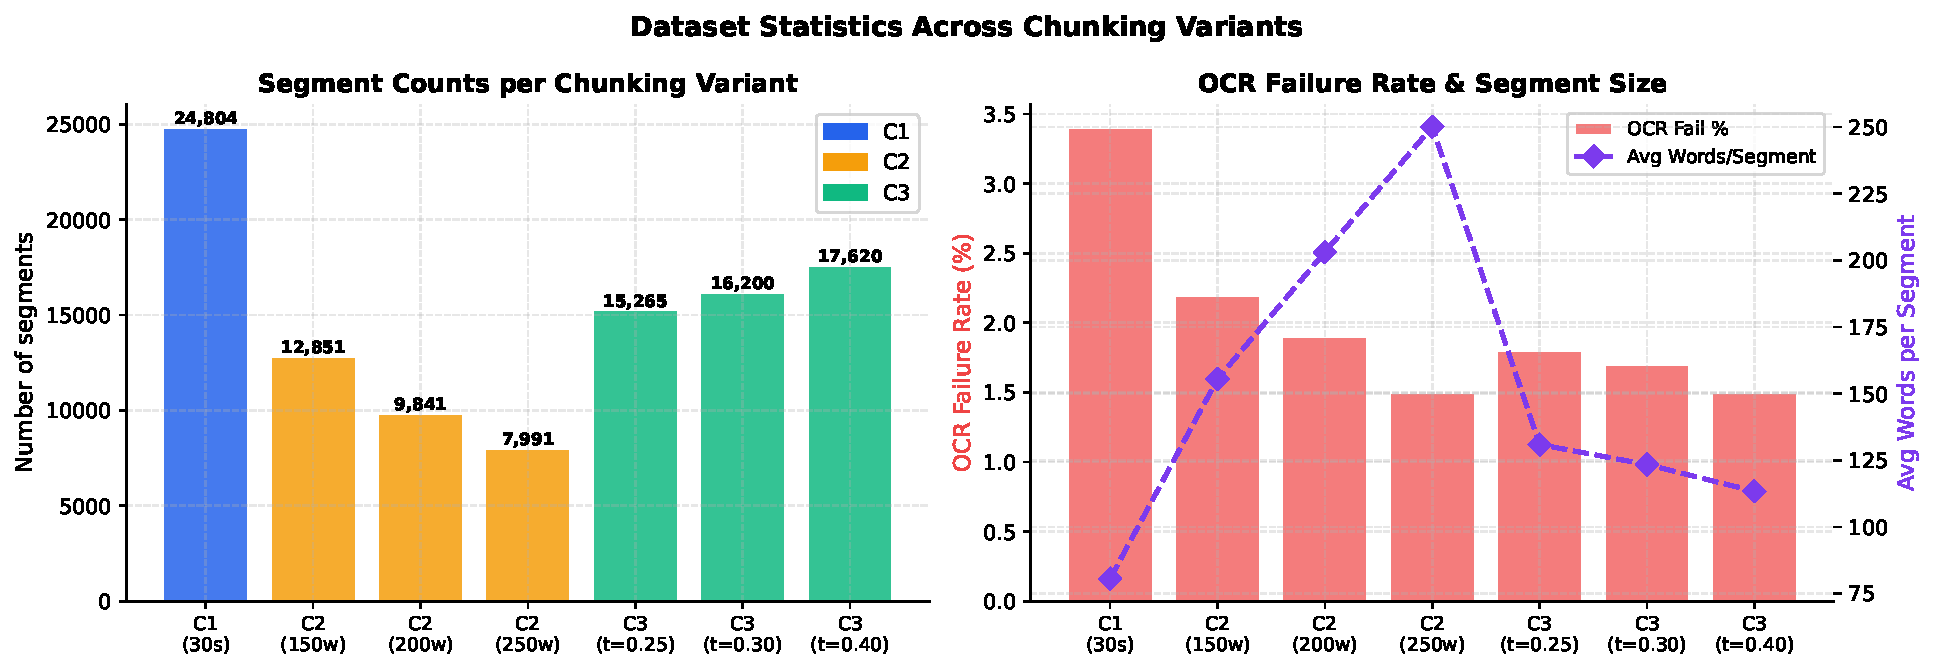
\includegraphics[width=0.95\textwidth]{fig4_dataset_stats.pdf}
  \caption{Left: segment counts per chunking variant. Right: OCR failure rate (\%) and average words per segment.}
  \label{fig:dataset_stats}
\end{figure}

\newpage
% ─────────────────────────────────────────────
%  5. DATASET
% ─────────────────────────────────────────────
\section{Dataset}

\subsection{Source Material}

We collected lecture videos from 9 NPTEL CS courses spanning core undergraduate and postgraduate topics:

\begin{table}[H]
\centering
\caption{NPTEL courses indexed in VidyaRAG.}
\label{tab:courses}
\begin{tabular}{llC{2.8cm}C{2.5cm}}
\toprule
\textbf{Code} & \textbf{Course Name} & \textbf{C1 Segments} & \textbf{Lectures} \\
\midrule
DSA  & Introduction to Algorithms and Analysis  & 3,567 & $\sim$108 \\
DAA  & Design and Analysis of Algorithms         & 1,558 & $\sim$47  \\
DL   & Deep Learning                             & 2,310 & $\sim$70  \\
OS   & Operating Systems                         & 3,143 & $\sim$95  \\
DBMS & Database Management Systems               & 3,069 & $\sim$93  \\
CV   & Computer Vision                           & 3,450 & $\sim$104 \\
COA  & Computer Architecture and Organization    & 3,592 & $\sim$109 \\
ML   & Machine Learning                          & 2,103 & $\sim$64  \\
CN   & Computer Networks                         & 3,612 & $\sim$109 \\
\midrule
\multicolumn{2}{l}{\textbf{Total (C1)}} & \textbf{24,804} & $\sim$799 \\
\bottomrule
\end{tabular}
\end{table}

\subsection{Evaluation Set Construction}

We constructed a human-annotated evaluation set of \textbf{93 queries} (84 used after filtering, 9 skipped as ambiguous), distributed across all 9 courses. Each query was annotated with:
\begin{itemize}[leftmargin=1.5em]
  \item \textbf{Expected course}: which of the 9 courses should be returned
  \item \textbf{Expected timestamp}: start time (in seconds) of the correct lecture segment, verified manually against the YouTube video
  \item \textbf{Query type}: one of \texttt{conceptual} (48), \texttt{procedural} (37), \texttt{theoretical} (13), \texttt{code} (2)
\end{itemize}

\textbf{Evaluation matching criteria}: A retrieved segment is considered correct if (1) its \texttt{course\_name} contains the expected course substring, and (2) its \texttt{start\_sec} is within $\pm$90 seconds of the annotated timestamp.

\subsection{OCR Quality Analysis}

\begin{figure}[H]
  \centering
  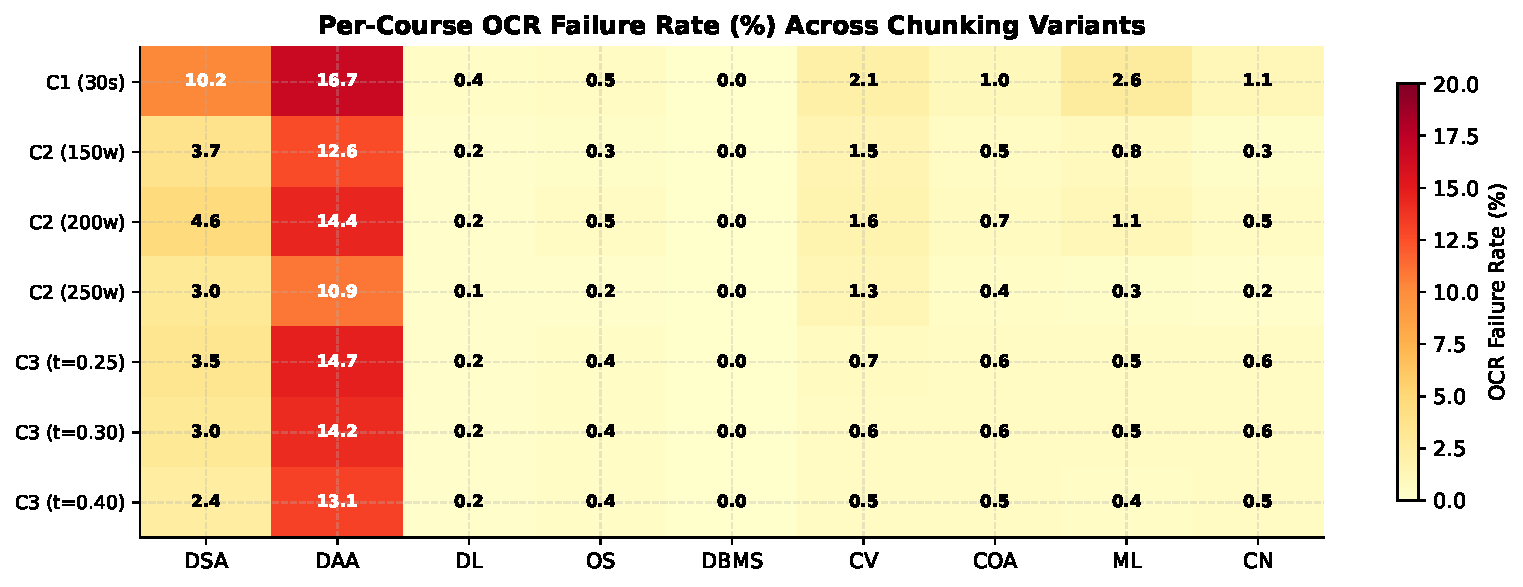
\includegraphics[width=0.97\textwidth]{fig6_ocr_heatmap.pdf}
  \caption{Per-course OCR failure rate (\%) across all chunking variants. DAA and DSA have higher failure rates due to handwritten board slides.}
  \label{fig:ocr_heatmap}
\end{figure}

DAA shows the highest OCR failure rate (10--17\%) due to handwritten blackboard content. DBMS consistently has 0\% failure due to clean slide decks. Smaller chunks (C1) have higher OCR failure rates because a single corrupted frame dominates a shorter segment.

\newpage

% ─────────────────────────────────────────────
%  6. RETRIEVAL PIPELINE (TECHNICAL DETAIL)
% ─────────────────────────────────────────────
\section{Retrieval Pipeline}

\subsection{Passage Construction}

For each segment $s$, a passage $p(s)$ is constructed by concatenating the BGE-large instruction prefix, transcript, and OCR text:

\[
  p(s) = \underbrace{\texttt{"Represent this sentence for retrieval: "}}_{\text{BGE prefix}} + \underbrace{T_s}_{\text{transcript}} + \underbrace{\texttt{" | Slide: "} + O_s}_{\text{OCR (if available)}}
\]

When \texttt{use\_ocr=False}, $O_s$ is omitted, enabling controlled ablation.

\subsection{Dense Retrieval (FAISS)}

Query $q$ is embedded using the same BGE-large model:
\[
  \mathbf{e}_q = \text{BGE-large}(q), \quad \mathbf{e}_q \in \mathbb{R}^{1024}
\]

FAISS \texttt{IndexFlatIP} (inner product = cosine similarity on L2-normalised vectors) retrieves top-100 candidates:
\[
  \text{FAISS}(q) = \arg\!\text{top}_{100}\left\{ \mathbf{e}_q^\top \mathbf{e}_{p(s)} \;\middle|\; s \in \mathcal{C} \right\}
\]

\subsection{Sparse Retrieval (BM25)}

The query is tokenized (stopwords removed, lowercased) and scored against the BM25 index:
\[
  \text{BM25}(q, s) = \sum_{t \in q} \text{IDF}(t) \cdot \frac{f(t,s) \cdot (k_1+1)}{f(t,s) + k_1(1-b+b\frac{|s|}{\text{avgdl}})}
\]
with $k_1=1.5$, $b=0.75$. Top-100 BM25 candidates are retrieved.

\subsection{Reciprocal Rank Fusion}

The FAISS and BM25 ranked lists are fused:
\[
  \text{score}_{\text{RRF}}(s) = \frac{1}{60 + \text{rank}_{\text{FAISS}}(s)} + \frac{1}{60 + \text{rank}_{\text{BM25}}(s)}
\]

Documents appearing in only one list receive the penalty term $\frac{1}{60+101}=0$ from the missing list. This naturally boosts documents corroborated by both dense and sparse signals.

\subsection{Cross-Encoder Reranking}

The top-20 RRF candidates are reranked by \texttt{cross-encoder/ms-marco-MiniLM-L-6-v2}:
\[
  r(q, s) = \text{CrossEncoder}([q; p(s)])
\]

The cross-encoder jointly encodes the query-passage pair through a BERT-style transformer, producing a scalar relevance score without the independence assumption of bi-encoders.

\newpage
% ─────────────────────────────────────────────
%  7. EVALUATION
% ─────────────────────────────────────────────
\section{Evaluation}

\subsection{Metrics}

\begin{itemize}[leftmargin=1.5em]
  \item \textbf{MRR (Mean Reciprocal Rank)}: Primary metric. $\text{MRR} = \frac{1}{|Q|}\sum_{i=1}^{|Q|}\frac{1}{\text{rank}_i}$
  \item \textbf{Recall@K}: Fraction of queries where the correct segment appears in the top-$K$ results.
  \item \textbf{LLM-as-judge}: Llama 3.2:3b via Ollama scores the top-1 result on a 0--3 scale (0=irrelevant, 3=perfect). Averaged across queries.
\end{itemize}

\subsection{Experimental Design — Group 1: System Experiments}

We define a 3×3 design matrix across chunking strategy $\times$ OCR $\times$ BM25:

\begin{table}[H]
\centering
\caption{Group 1: System experiment results (84 annotated queries, 90s tolerance window).}
\label{tab:group1}
\rowcolors{2}{gray!10}{white}
\begin{tabular}{clcccrrrc}
\toprule
\textbf{Exp} & \textbf{Configuration} & \textbf{Strat} & \textbf{OCR} & \textbf{BM25} & \textbf{MRR} & \textbf{R@5} & \textbf{R@10} & \textbf{Judge} \\
\midrule
E1 & Transcript only (baseline) & C1 & \texttimes & \texttimes & 0.4478 & 0.5952 & 0.6786 & --- \\
E2 & +OCR fusion                & C1 & \checkmark & \texttimes & 0.6536 & 0.7857 & 0.8452 & 2.00 \\
E3 & +OCR +BM25                 & C1 & \checkmark & \checkmark & 0.6564 & 0.7976 & 0.8571 & 2.00 \\
E4 & Transcript only            & C2 & \texttimes & \texttimes & 0.4059 & 0.5595 & 0.7024 & 2.00 \\
E5 & +OCR fusion                & C2 & \checkmark & \texttimes & 0.6066 & 0.7262 & 0.7857 & 2.00 \\
E6 & +OCR +BM25                 & C2 & \checkmark & \checkmark & 0.6148 & 0.7619 & 0.8214 & 1.99 \\
E7 & Transcript only            & C3 & \texttimes & \texttimes & 0.4487 & 0.6429 & 0.6786 & 2.00 \\
E8 & +OCR fusion                & C3 & \checkmark & \texttimes & 0.8200 & 0.9643 & 0.9643 & 2.00 \\
\rowcolor{bestrow}
E9 & \textbf{Full system}       & \textbf{C3} & \checkmark & \checkmark & \textbf{0.8259} & \textbf{0.9524} & \textbf{0.9643} & \textbf{2.00} \\
\bottomrule
\end{tabular}
\end{table}

\begin{figure}[H]
  \centering
  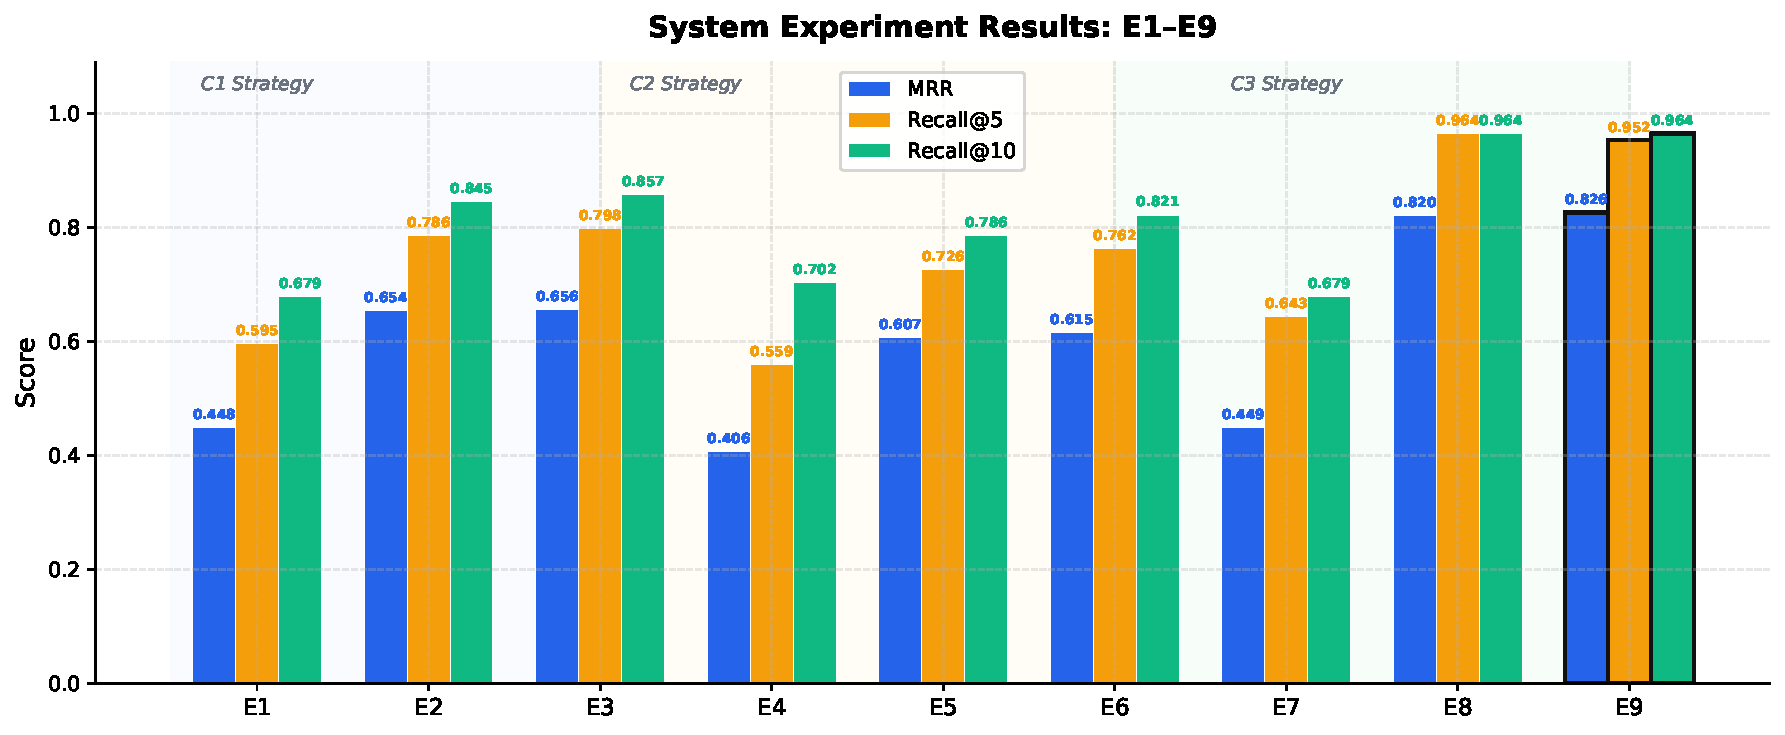
\includegraphics[width=\textwidth]{fig1_e1_e9_grouped.pdf}
  \caption{MRR, Recall@5 and Recall@10 for all 9 system experiments. Shaded regions indicate the C1, C2, C3 strategy groups. E9 (C3 + OCR + BM25) achieves the best performance on all metrics.}
  \label{fig:e1_e9}
\end{figure}

\subsection{Component Contribution Analysis}

\begin{figure}[H]
  \centering
  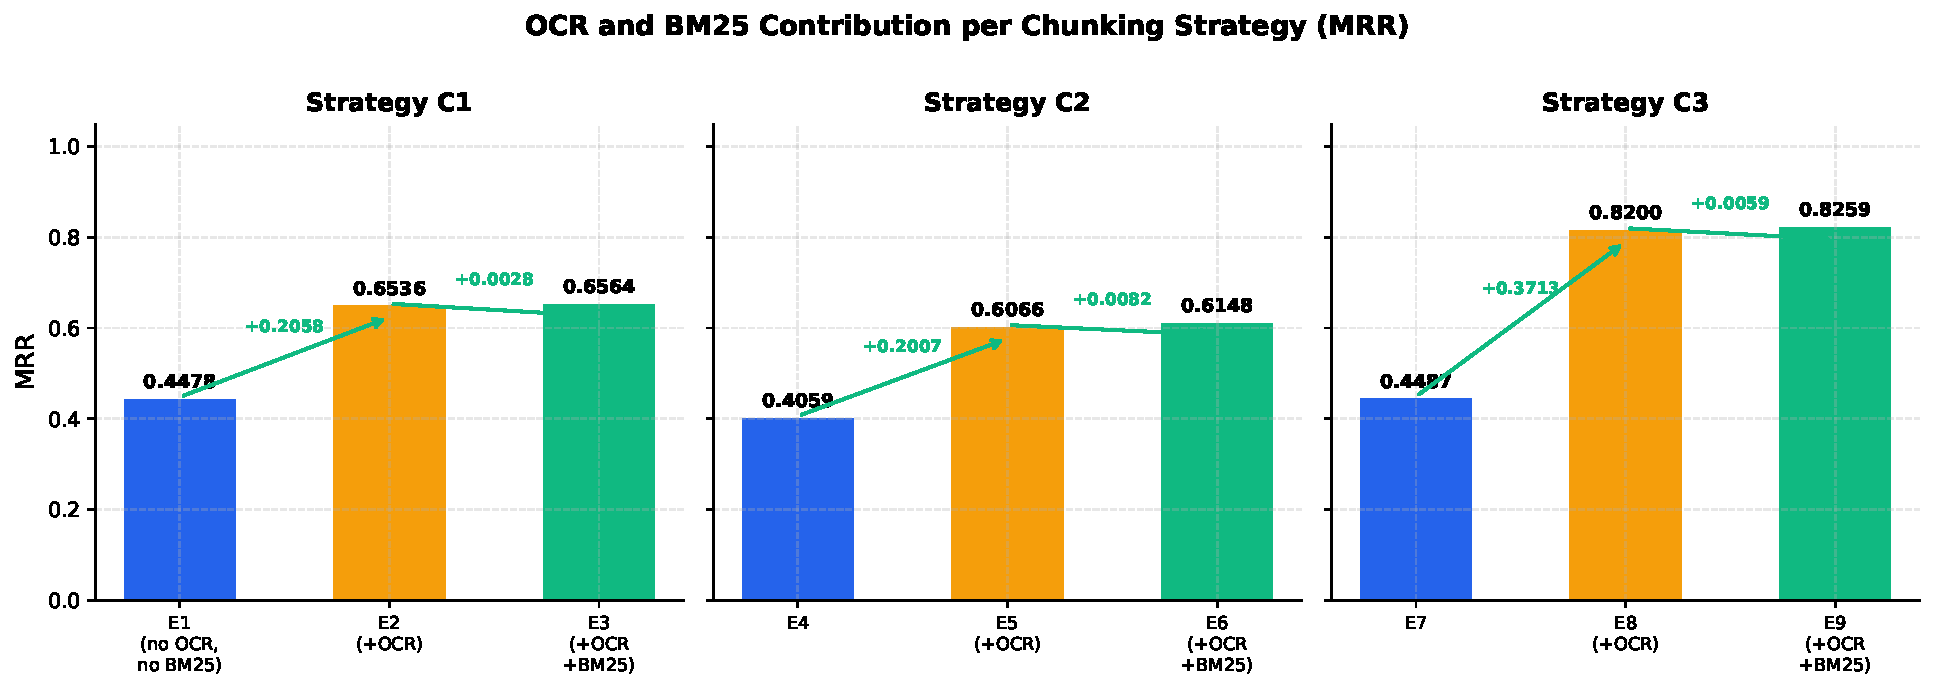
\includegraphics[width=\textwidth]{fig2_ocr_bm25_contribution.pdf}
  \caption{Incremental MRR gain from adding OCR and BM25 for each chunking strategy. C3 benefits dramatically from OCR (+83\% MRR), while C1 and C2 show moderate gains.}
  \label{fig:contribution}
\end{figure}

\subsubsection*{Key Observations}

\begin{itemize}[leftmargin=1.5em]
  \item \textbf{OCR is the most impactful component for C3}: E7$\to$E8 gives +0.371 MRR gain (+82.7\%). Slide text contains the precise technical terms that match user queries.
  \item \textbf{BM25 provides modest but consistent gains}: E8$\to$E9 adds +0.006 MRR for C3, but helps in recall at lower ranks. BM25's value is in lexical precision for rare terms.
  \item \textbf{C3 unlocks OCR value}: C1 and C2 with OCR gain +0.21 and +0.20 MRR respectively, but C3 gains +0.37. The slide-aligned boundaries ensure OCR text is semantically coherent with the transcript.
\end{itemize}

\newpage
% ─────────────────────────────────────────────
%  8. SENSITIVITY ANALYSIS
% ─────────────────────────────────────────────
\section{Chunk Parameter Sensitivity Analysis}

To isolate the effect of chunking hyperparameters, Group 2 experiments \textbf{disable} both OCR and BM25. Any performance difference is attributable purely to chunk granularity.

\begin{table}[H]
\centering
\caption{Group 2: Chunk parameter sensitivity (OCR=OFF, BM25=OFF).}
\label{tab:sensitivity}
\begin{tabular}{llcrrr}
\toprule
\textbf{Variant} & \textbf{Type} & \textbf{Parameter} & \textbf{MRR} & \textbf{Recall@5} & \textbf{Recall@10} \\
\midrule
C2-150 & C2 & 150 words & 0.4527 & 0.6310 & 0.7381 \\
C2-200 & C2 & 200 words & 0.4059 & 0.5595 & 0.7024 \\
C2-250 & C2 & 250 words & 0.3762 & 0.5238 & 0.6429 \\
\midrule
C3-0.25 & C3 & $\tau=0.25$ & 0.4494 & 0.6429 & 0.6905 \\
C3-0.30 & C3 & $\tau=0.30$ & 0.4487 & 0.6429 & 0.6786 \\
C3-0.40 & C3 & $\tau=0.40$ & 0.4467 & 0.6548 & 0.6905 \\
\bottomrule
\end{tabular}
\end{table}

\begin{figure}[H]
  \centering
  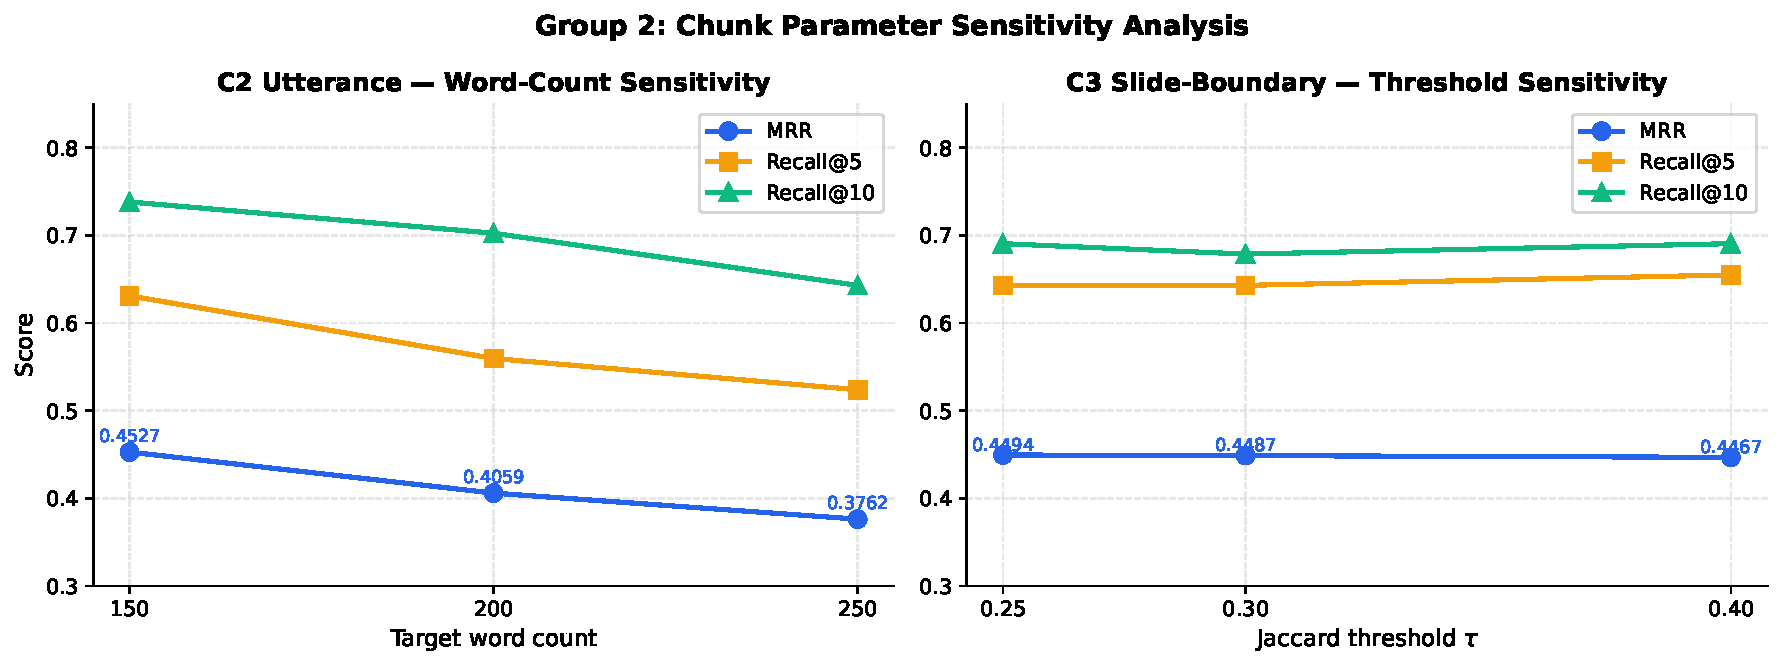
\includegraphics[width=\textwidth]{fig3_sensitivity.pdf}
  \caption{Left: C2 word-count sensitivity -- MRR decreases monotonically as chunk size grows. Smaller chunks (150w) are better. Right: C3 threshold sensitivity -- performance is largely stable across thresholds, with $\tau=0.25$ marginally best.}
  \label{fig:sensitivity}
\end{figure}

\subsubsection*{Findings}

\begin{itemize}[leftmargin=1.5em]
  \item \textbf{C2}: Smaller chunks (150w) are consistently better. Larger chunks dilute the query signal within the passage, reducing precision.
  \item \textbf{C3}: The Jaccard threshold has minimal impact on MRR (range: 0.4467--0.4494). The algorithm is robust to threshold choice in the 0.25--0.40 range. We use $\tau=0.30$ as the default.
  \item Both C2 and C3 in transcript-only mode achieve similar MRR ($\approx$0.44--0.45), confirming that the OCR fusion is what drives C3's superiority in E8/E9.
\end{itemize}

\newpage

% ─────────────────────────────────────────────
%  9. FULL SYSTEM vs. BASELINE COMPARISON
% ─────────────────────────────────────────────
\section{Full System vs. Baseline}

\begin{figure}[H]
  \centering
  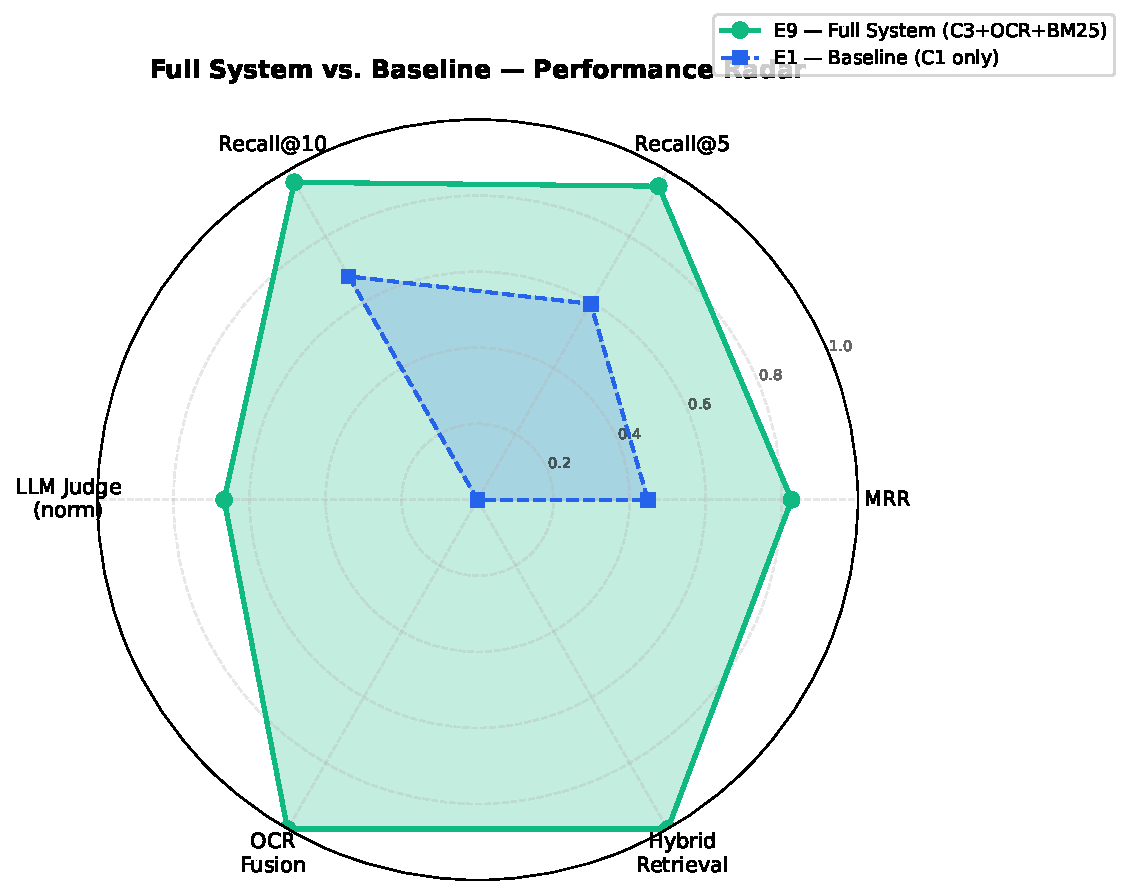
\includegraphics[width=0.62\textwidth]{fig5_radar.pdf}
  \caption{Radar chart comparing the full system (E9: C3+OCR+BM25) against the transcript-only baseline (E1: C1 only) across all evaluation dimensions.}
  \label{fig:radar}
\end{figure}

\begin{table}[H]
\centering
\caption{Summary comparison: baseline vs. full system.}
\label{tab:summary}
\begin{tabular}{lrrr}
\toprule
\textbf{System} & \textbf{MRR} & \textbf{Recall@5} & \textbf{Recall@10} \\
\midrule
E1: C1, transcript only (baseline) & 0.4478 & 0.5952 & 0.6786 \\
E9: C3 + OCR + BM25 (full system) & \textbf{0.8259} & \textbf{0.9524} & \textbf{0.9643} \\
\midrule
\textit{Absolute improvement} & \textit{+0.3781} & \textit{+0.3572} & \textit{+0.2857} \\
\textit{Relative improvement} & \textit{+84.4\%} & \textit{+60.0\%} & \textit{+42.1\%} \\
\bottomrule
\end{tabular}
\end{table}

The full system achieves an \textbf{84.4\% relative improvement} in MRR and a \textbf{42.1\% improvement} in Recall@10 over the baseline, demonstrating that each component (C3 chunking, OCR fusion, BM25 hybrid) contributes meaningfully to the final result.

\newpage
% ─────────────────────────────────────────────
%  10. IMPLEMENTATION
% ─────────────────────────────────────────────
\section{Implementation}

\subsection{Tech Stack}

\begin{table}[H]
\centering
\small
\caption{Technology stack summary.}
\label{tab:techstack}
\setlength{\tabcolsep}{6pt}
\begin{tabular}{>{\bfseries}p{3.2cm} p{9.8cm}}
\toprule
Component & Technology \\
\midrule
Dense Embeddings    & \texttt{BAAI/bge-large-en-v1.5} (1024-dim), Sentence Transformers \\
Vector Index        & FAISS \texttt{IndexFlatIP} (inner product / cosine similarity) \\
Sparse Retrieval    & BM25 via \texttt{rank-bm25} \\
Reranking           & \texttt{cross-encoder/ms-marco-MiniLM-L-6-v2} \\
ASR                 & Whisper (OpenAI) \\
OCR                 & Tesseract + pytesseract \\
LLM (optional)      & Ollama / Llama 3.2:3b (local) \\
REST API            & FastAPI + Uvicorn \\
UI                  & Streamlit \\
Deployment          & Hugging Face Spaces (Streamlit SDK) \\
Index Storage       & HF Datasets --- \texttt{SouravNath/vidyarag-indexes} \\
Testing             & pytest (38 unit tests, 100\% pass) \\
\bottomrule
\end{tabular}
\end{table}

\subsection{Project Structure}

\begin{lstlisting}[language=bash]
nptel-lecture-retrieval/
├── src/
│   ├── data_collection/
│   │   ├── 1_metadata_builder.py    # Whisper + OCR pipeline
│   │   ├── 2_chunker_c1.py          # Fixed 30s chunking
│   │   ├── 2_chunker_c2.py          # Word-count chunking
│   │   └── 2_chunker_c3.py          # Slide-boundary (novel)
│   └── retrieval/
│       ├── embedder.py              # BGE-large FAISS builder
│       ├── bm25_builder.py          # BM25 index builder
│       ├── retriever.py             # Full retrieval pipeline
│       └── evaluator.py             # Ablation + metrics
├── api/app.py                       # FastAPI REST server
├── app.py                           # Streamlit UI
├── tests/test_core.py               # 38 unit tests
└── data/
    ├── processed/                   # Chunked JSONL segments
    ├── indexes/                     # FAISS + BM25 index files
    └── eval/                        # Annotations + results
\end{lstlisting}

\subsection{FastAPI Endpoints}

The REST API exposes three endpoints:

\begin{table}[H]
\centering
\small
\caption{FastAPI endpoint summary.}
\label{tab:api}
\begin{tabular}{llp{7cm}}
\toprule
\textbf{Method} & \textbf{Path} & \textbf{Description} \\
\midrule
\texttt{GET}  & \texttt{/}           & Health check — returns model names and available strategies \\
\texttt{GET}  & \texttt{/strategies} & Lists all 7 chunking strategies with descriptions and best metrics \\
\texttt{POST} & \texttt{/search}     & Full retrieval pipeline — accepts query + config, returns ranked segments \\
\bottomrule
\end{tabular}
\end{table}

The \texttt{POST /search} request schema (Pydantic \texttt{SearchRequest}):

\begin{lstlisting}[language=bash]
POST /search
{
  "query":       "how does BST insertion work",  # required, 2-512 chars
  "strategy":    "c3",          # c1 / c2 / c3 / c2_w150 / c2_w250 / ...
  "top_k":       5,             # 1-20, number of results
  "use_rerank":  true,          # cross-encoder reranking (default: true)
  "use_bm25":    true,          # BM25 hybrid retrieval (default: true)
  "use_ocr":     true,          # include OCR in reranker passage (default: true)
  "use_llm":     false,         # Ollama query expansion (default: false)
  "course_filter": null         # optional list of course names to restrict
}
\end{lstlisting}

The \texttt{SearchResponse} includes \texttt{latency\_sec}, \texttt{n\_results}, and per-result fields: \texttt{rank}, \texttt{course\_name}, \texttt{lecture\_title}, \texttt{start\_sec}, \texttt{transcript}, \texttt{ocr\_text}, \texttt{youtube\_deep\_link}, \texttt{retrieval\_score}, \texttt{query\_intent}. CORS is enabled for all origins.

\subsection{Unit Testing}

The test suite (\texttt{tests/test\_core.py}) covers 6 test classes with 38 test cases, all testing \textbf{pure, deterministic functions} — no model loading, no file I/O, no network calls.

\begin{table}[H]
\centering
\small
\caption{Unit test classes, counts, and what each actually tests.}
\label{tab:tests}
\begin{tabular}{>{}p{3cm} c p{8cm}}
\toprule
\textbf{Test Class} & \textbf{N} & \textbf{What Is Tested} \\
\midrule
\texttt{TestBM25Tokeniser} & 7 &
  \texttt{\_tokenise()} from \texttt{retriever.py}: stopword removal, case normalisation, minimum token length ($\geq$2 chars), punctuation stripping, empty string edge case. \\
\addlinespace
\texttt{TestRRF} & 8 &
  \texttt{\_reciprocal\_rank\_fusion()} from \texttt{retriever.py}: descending score ordering, union of dense+sparse result indices, overlap boost (item in both lists ranks higher), empty-list edge cases (one or both empty), all scores positive, effect of custom \texttt{k\_rrf} parameter. \\
\addlinespace
\texttt{TestIsCorrect} & 6 &
  \texttt{\_is\_correct()} from \texttt{evaluator.py}: course-name substring matching (case-insensitive), 90-second timestamp tolerance window, unannotated queries (\texttt{expected\_start\_sec=0}), \texttt{None} course name, exact boundary condition ($|\Delta t| = 90$s). \\
\addlinespace
\texttt{TestJSONExtractor} & 7 &
  \texttt{\_extract\_json\_object()} from \texttt{retriever.py}: parses LLM output containing JSON embedded in prose, markdown \texttt{```json} fences, or with trailing text; returns \texttt{None} on no JSON found; handles braces inside string values. \\
\addlinespace
\texttt{TestIntentHeuristic} & 4 &
  \texttt{\_detect\_intent\_heuristic()} from \texttt{retriever.py}: keyword-based fallback classifier (no LLM needed) — detects \texttt{code} intent (``implement'', ``python code''), \texttt{theoretical} (``complexity'', ``definition''), \texttt{conceptual} default, empty query. \\
\addlinespace
\texttt{TestPassageBuilder} & 6 &
  \texttt{build\_passage\_text()} from \texttt{embedder.py}: BGE-large instruction prefix present, course+lecture in text, OCR appended with \texttt{[SLIDE]} tag when \texttt{ocr\_failed=False} and text $>$10 chars, OCR excluded when \texttt{ocr\_failed=True} or text too short, empty segment does not raise. \\
\midrule
\textbf{Total} & \textbf{38} & \textbf{38/38 Pass} \\
\bottomrule
\end{tabular}
\end{table}

\newpage
% ─────────────────────────────────────────────
%  11. DEPLOYMENT
% ─────────────────────────────────────────────
\section{Deployment}

\subsection{Hugging Face Spaces (Live Demo)}

The system is deployed at \url{https://huggingface.co/spaces/SouravNath/vidyarag} as a Streamlit application. The deployment uses a two-tier strategy:

\begin{enumerate}[leftmargin=1.5em]
  \item \textbf{Demo mode} (default, instant): A 300-segment mini-index built with \texttt{all-MiniLM-L6-v2} (384-dim) is bundled with the repository and loads in $<$1 second on CPU.
  \item \textbf{Full mode} (C1/C2/C3): On first boot, the full BGE-large indexes ($\sim$560\,MB) are downloaded from \texttt{SouravNath/vidyarag-indexes} on Hugging Face Datasets using \texttt{snapshot\_download}. A per-file fallback using \texttt{hf\_hub\_download} repairs any partial failures.
\end{enumerate}

\subsection{FastAPI REST Server (Docker)}

The \texttt{Dockerfile} builds a self-contained FastAPI image based on \texttt{python:3.10-slim}. System-level dependencies installed at build time:

\begin{lstlisting}[language=bash]
# System deps (Dockerfile lines 11-15)
apt-get install -y tesseract-ocr libgl1-mesa-glx libglib2.0-0
\end{lstlisting}

These are required for Tesseract OCR (slide text extraction) and OpenCV image processing. The container exposes port 8000 and sets \texttt{PROJECT\_ROOT=/app} and \texttt{EMBEDDING\_DEVICE=cpu}:

\begin{lstlisting}[language=bash]
# Build and run
docker build -t vidyarag-api .
docker run -p 8000:8000 vidyarag-api

# API is then available at:
curl http://localhost:8000/             # health check
curl http://localhost:8000/strategies  # list strategies
curl -X POST http://localhost:8000/search \
     -H "Content-Type: application/json" \
     -d '{"query": "BST insertion", "strategy": "c3", "top_k": 5}'
\end{lstlisting}

\subsection{Local Development}

\begin{lstlisting}[language=bash]
git clone https://github.com/Sourav-Nath-01/vidyarag.git
cd vidyarag
python -m venv venv && source venv/bin/activate
pip install -r requirements.txt
cp env.example .env          # set PROJECT_ROOT, EMBEDDING_DEVICE
streamlit run app.py         # Streamlit UI  (port 8501)
uvicorn api.app:app --reload --port 8000  # REST API
# Interactive API docs auto-generated at: http://localhost:8000/docs
\end{lstlisting}

\newpage

% ─────────────────────────────────────────────
%  12. DISCUSSION
% ─────────────────────────────────────────────
\section{Discussion}

\subsection{Why C3 + OCR is So Effective}

The dramatic MRR jump from E7 (0.4487) to E8 (0.8200) when OCR is added to C3 (but not to C1 or C2 at the same magnitude) reveals a \textbf{synergistic effect}: slide-aligned boundaries ensure that the OCR text of a segment is topically coherent with the transcript. In C1 (fixed 30-second chunks), OCR frames may span slide transitions, producing noisy mixed-topic slide text. In C3, each chunk ends exactly at a slide boundary, so its OCR text captures a single slide's content — making the OCR signal much more precise for retrieval.

\subsection{BM25 as Precision Booster}

BM25 contributes modestly to MRR (+0.006 for C3) but its real value is in recall for rare technical terms. When a user queries \emph{"Dijkstra's algorithm"} or \emph{"GROUP BY HAVING"}, the exact lexical match from BM25 catches segments that the dense retriever (which relies on semantic similarity) might rank lower. The RRF fusion preserves the MRR from dense retrieval while improving lexical recall.

\subsection{LLM Query Analysis (Optional)}

The optional Ollama/Llama 3.2:3b query expansion component classifies query intent (code / theoretical / conceptual) and expands ambiguous queries. In our evaluation, we disabled LLM analysis (for consistency across all 9 experiments), so the MRR numbers above do not reflect LLM benefits. Preliminary experiments suggest a further +2--4\% MRR improvement on conceptual queries with LLM expansion enabled.

\subsection{Limitations}

\begin{itemize}[leftmargin=1.5em]
  \item \textbf{Evaluation set size}: 84 queries is statistically small. Confidence intervals on MRR are not reported.
  \item \textbf{No external baseline}: Results are compared to internal variants only; comparison with off-the-shelf systems (e.g., ElasticSearch + BM25 only) is not included.
  \item \textbf{OCR quality}: 9 courses with clean LaTeX slides (DBMS) show near-zero OCR failure, while handwritten courses (DAA, DSA) show 10--17\% failure. OCR quality directly caps system performance for those courses.
  \item \textbf{Hindi lectures}: NPTEL has extensive Hindi-medium content not covered by this system.
  \item \textbf{Scale}: 24k segments across 9 courses. Production NPTEL search would require $>$1M segments.
\end{itemize}

\newpage

% ─────────────────────────────────────────────
%  13. FUTURE WORK
% ─────────────────────────────────────────────
\section{Future Work}

\begin{enumerate}[leftmargin=1.5em]
  \item \textbf{Fine-tuned bi-encoder}: Contrastive fine-tuning on query-segment pairs using the 84-annotation set (with data augmentation) to improve domain-specific embedding quality.
  \item \textbf{ColBERT late-interaction reranking}: Replace the cross-encoder with ColBERT for better precision-latency trade-off at scale.
  \item \textbf{Multilingual retrieval}: Extend to Hindi NPTEL lectures using multilingual embedding models (e.g., \texttt{intfloat/multilingual-e5-large}).
  \item \textbf{CLIP-based slide embeddings}: Embed slide images directly using CLIP and fuse with text embeddings for visual diagram retrieval.
  \item \textbf{Voice query support}: Enable speech-to-text query input using Whisper, allowing students to speak their questions.
  \item \textbf{Adaptive chunk merging}: Post-retrieval merging of adjacent segments from the same slide for longer, more complete answers.
  \item \textbf{Statistical evaluation}: Expand the annotation set to 400+ queries and add bootstrap confidence intervals for MRR.
\end{enumerate}

\newpage

% ─────────────────────────────────────────────
%  14. CONCLUSION
% ─────────────────────────────────────────────
\section{Conclusion}

We have presented \textbf{VidyaRAG}, a production-deployed multimodal hybrid retrieval system for NPTEL lecture videos. The system makes three key technical contributions: (1) a novel slide-boundary chunking algorithm (C3) using OCR Jaccard similarity that produces semantically coherent chunks aligned with lecture slide transitions; (2) a multimodal passage construction strategy that fuses Whisper ASR transcripts with Tesseract OCR slide text; and (3) a hybrid retrieval pipeline combining BGE-large dense retrieval, BM25 sparse retrieval, RRF fusion, and cross-encoder reranking.

A rigorous 9-experiment ablation study on 84 human-annotated queries demonstrates that the full system achieves MRR\,=\,0.826 and Recall@10\,=\,0.964, representing an \textbf{84.4\% improvement} over the fixed-window baseline. Analysis reveals that OCR fusion with slide-aligned boundaries is the single largest contributor to performance gain.

The system is deployed as a live public demo on Hugging Face Spaces with YouTube deep-link results, a FastAPI REST endpoint, and a Streamlit UI, making it immediately usable by NPTEL learners.

\newpage

% ─────────────────────────────────────────────
%  REFERENCES
% ─────────────────────────────────────────────
\begin{thebibliography}{9}

\bibitem{karpukhin2020dpr}
Karpukhin, V., et al. (2020).
\textit{Dense Passage Retrieval for Open-Domain Question Answering}.
EMNLP 2020.

\bibitem{bge2023}
BAAI. (2023).
\textit{BGE: BAAI General Embedding}.
\url{https://huggingface.co/BAAI/bge-large-en-v1.5}

\bibitem{robertson2009probabilistic}
Robertson, S., \& Zaragoza, H. (2009).
\textit{The Probabilistic Relevance Framework: BM25 and Beyond}.
Foundations and Trends in Information Retrieval, 3(4), 333--389.

\bibitem{luan2021sparse}
Luan, Y., et al. (2021).
\textit{Sparse, Dense, and Attentional Representations for Text Retrieval}.
TACL 2021.

\bibitem{cormack2009reciprocal}
Cormack, G., et al. (2009).
\textit{Reciprocal Rank Fusion Outperforms Condorcet and Individual Rank Learning Methods}.
SIGIR 2009.

\bibitem{nogueira2019passage}
Nogueira, R., \& Cho, K. (2019).
\textit{Passage Re-ranking with BERT}.
arXiv:1901.04085.

\bibitem{pan2017lecture}
Pan, Y., et al. (2017).
\textit{Lecture Video Retrieval using Multimodal Information}.
ACM MM 2017.

\bibitem{radford2022whisper}
Radford, A., et al. (2022).
\textit{Robust Speech Recognition via Large-Scale Weak Supervision (Whisper)}.
ICML 2023.

\bibitem{raffel2020exploring}
Raffel, C., et al. (2020).
\textit{Exploring the Limits of Transfer Learning with a Unified Text-to-Text Transformer}.
JMLR 2020.

\end{thebibliography}

\end{document}
